\documentclass[pdflatex,compress,mathserif]{beamer}

%\usetheme[dark,framenumber,totalframenumber]{ElektroITK}
\usetheme[darktitle,framenumber,totalframenumber]{ElektroITK}

\usepackage[utf8]{inputenc}
\usepackage[T1]{fontenc}
\usepackage{lmodern}
\usepackage[bahasai]{babel}
\usepackage{amsmath}
\usepackage{amsfonts}
\usepackage{amssymb}
\usepackage{graphicx}
\usepackage{multicol}
\usepackage{lipsum}
\usefonttheme[onlymath]{serif}

\newcommand*{\Scale}[2][4]{\scalebox{#1}{$#2$}}%

\setbeamertemplate{caption}[numbered]

\title{Kecerdasan Buatan}
\subtitle{Neural Network}

\author{Mifta Nur Farid}

\date{29 Februari 2024}

\begin{document}

\maketitle

\begin{frame}{Neural Network}
	\begin{center}
		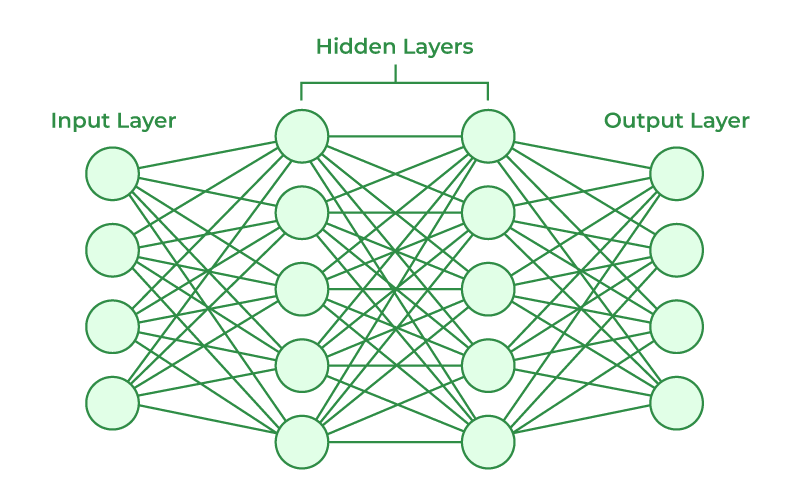
\includegraphics[width=\linewidth]{img/16}
	\end{center}
\end{frame}

\begin{frame}{Simplest Neural Network}
	\begin{center}
		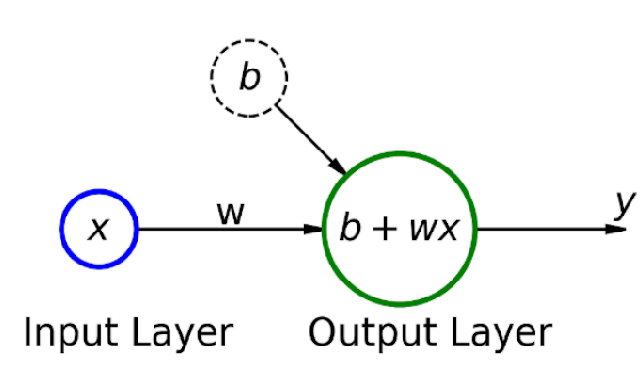
\includegraphics[width=0.6\linewidth]{img/15}
	\end{center}
\end{frame}

\begin{frame}{Regression Problem}
	\begin{multicols}{2}
		\begin{center}
			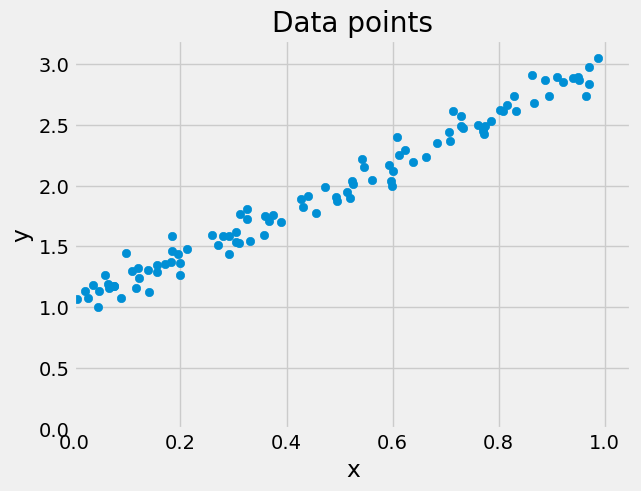
\includegraphics[width=\linewidth]{img/01}
		\end{center}
		\columnbreak
		model:
		$y = b + wx$
		\begin{align*}
			y &: \text{label } y \\
			x &: \text{feature } x \\
			b &: \text{parameter bias} \\
			w &: \text{parameter weight}
		\end{align*}
		\vfill\null
	\end{multicols}
\end{frame}

\begin{frame}{Regression Problem}
	\begin{multicols}{2}
		\begin{center}
			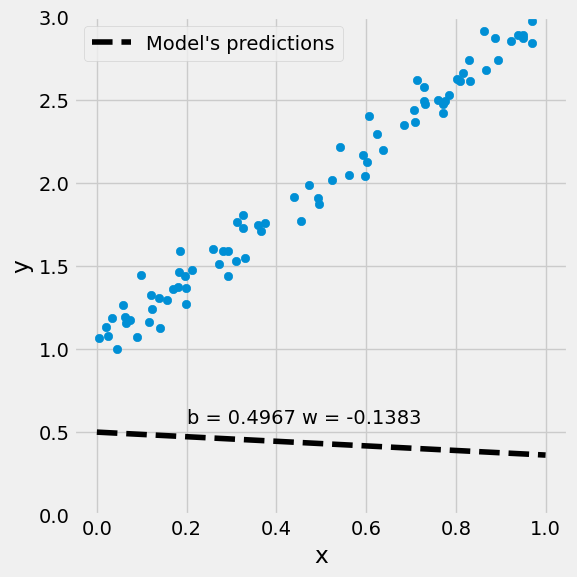
\includegraphics[width=\linewidth]{img/03}
		\end{center}
		\columnbreak
		\begin{itemize}
			\item randomly initialize the parameters $b$ and $w$
		\end{itemize}
	\end{multicols}
\end{frame}

\begin{frame}{Regression Problem}
	\begin{multicols}{2}
		\begin{center}
			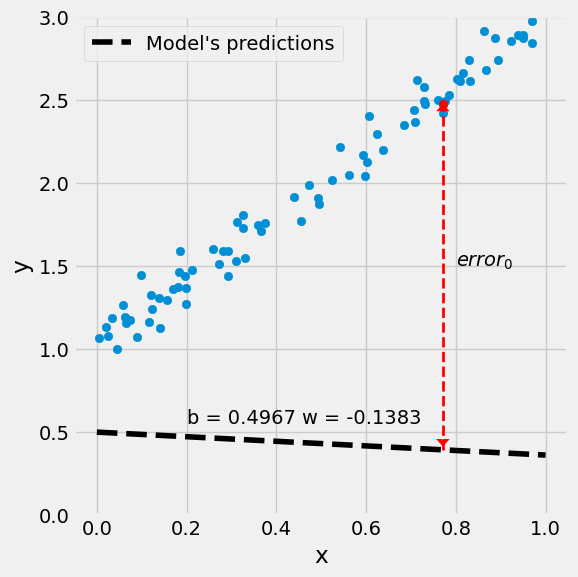
\includegraphics[width=\linewidth]{img/04}
		\end{center}
		\columnbreak
		\begin{itemize}
			\item Computer the loss $\text{error}_i = \bar{y}_i - y_i$
			\item \textbf{Batch} gradient descent: all points ($n = N$)
			\item \textbf{Stochastic} gradient descent: single point ($n = 1$)
			\item \textbf{Mini-batch} gradient descent: anything else ($1 < n < N$)
		\end{itemize}
	\end{multicols}
\end{frame}

\begin{frame}{Regression Problem}
	\begin{multicols}{2}
		\begin{center}
			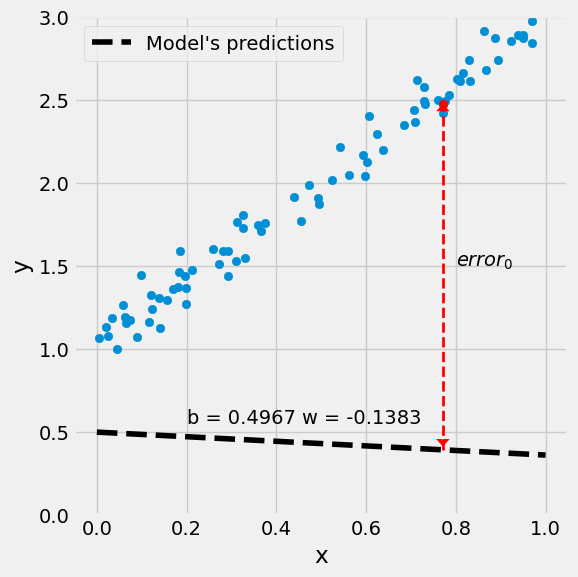
\includegraphics[width=\linewidth]{img/04}
		\end{center}
		\columnbreak
		\begin{itemize}
			\item Loss = aggregation of errors for a set of data points
			\item For a regression problem, the loss is given by the mean squared error (MSE)
		\end{itemize}
		$$
		\begin{aligned}
			\text{MSE} &= \frac{1}{n} \sum_{i=1}^n{\text{error}_i}^2
			\\
			&= \frac{1}{n} \sum_{i=1}^n{(\hat{y_i} - y_i)}^2
			\\
			&= \frac{1}{n} \sum_{i=1}^n{(b + w x_i - y_i)}^2
		\end{aligned}
		$$
	\end{multicols}
\end{frame}

\begin{frame}{Regression Problem}
	\begin{itemize}
		\item What if we did the same for ALL possible values of $b$ and $w$?
	\end{itemize}
	\begin{center}
		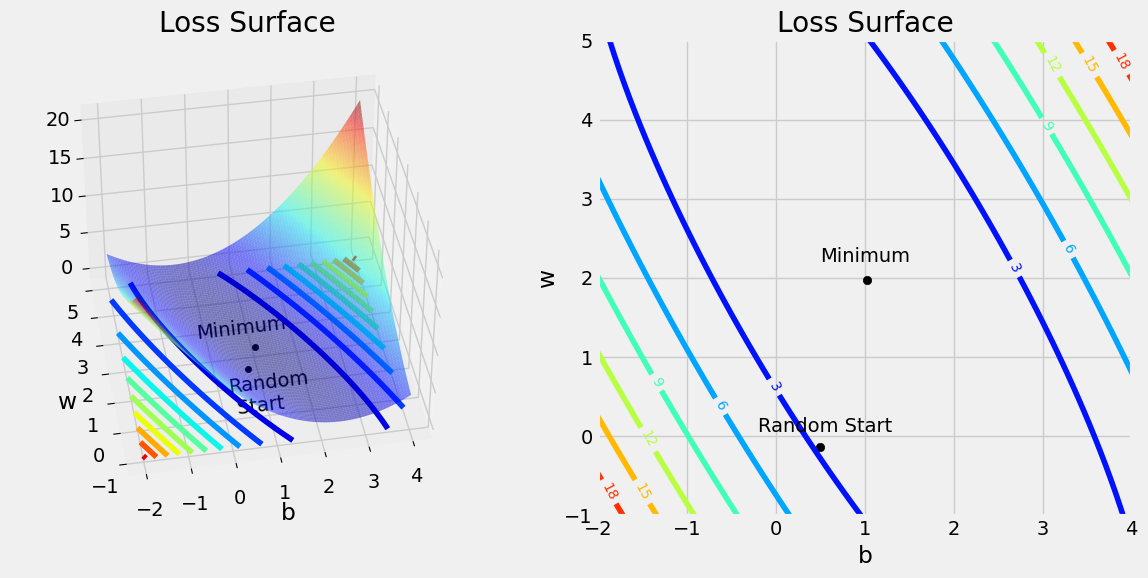
\includegraphics[width=\linewidth]{img/05}
	\end{center}
\end{frame}

\begin{frame}{Regression Problem}
	\begin{center}
		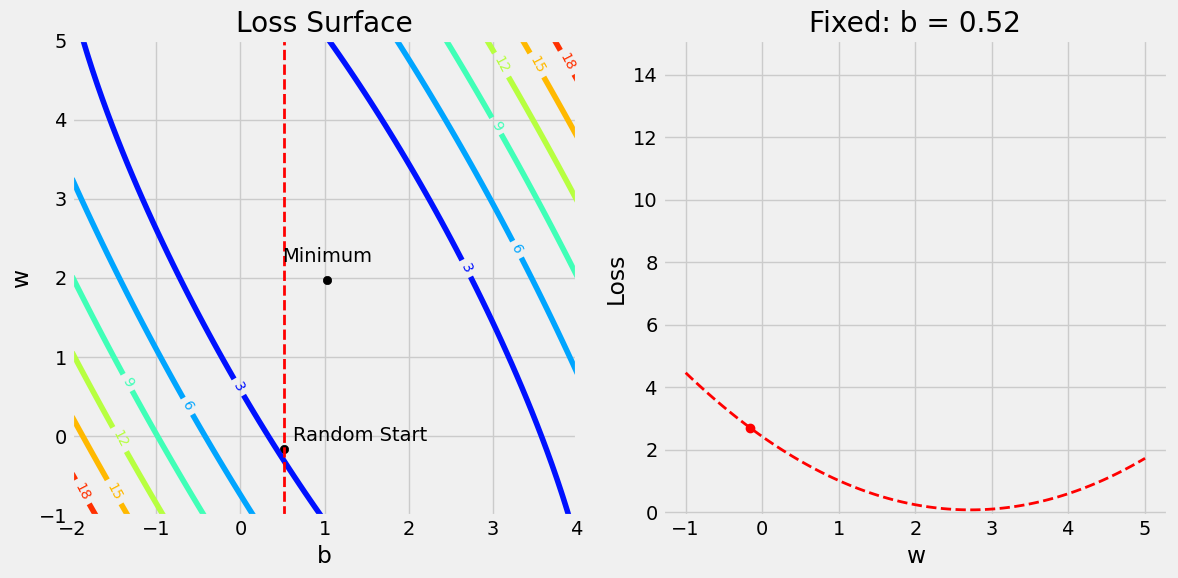
\includegraphics[width=\linewidth]{img/06}
	\end{center}
\end{frame}

\begin{frame}{Regression Problem}
	\begin{center}
		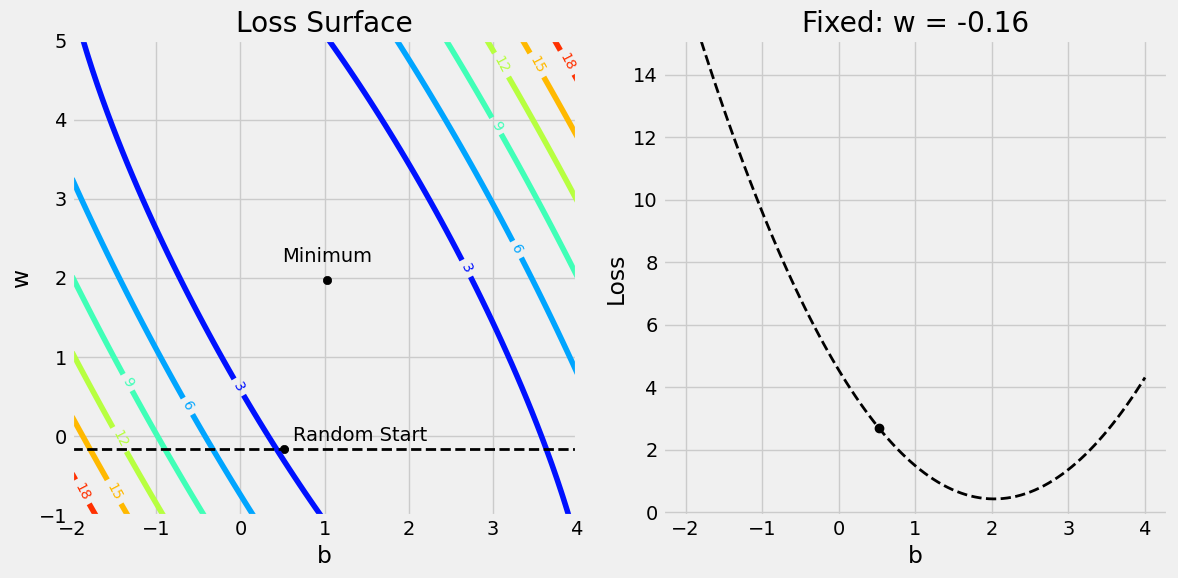
\includegraphics[width=\linewidth]{img/07}
	\end{center}
\end{frame}

\begin{frame}{Regression Problem}
	\begin{itemize}
		\item Compute the Gradients
		\item Gradient : how much the loss changes if ONE parameter changes a little bit
		\item Gradient $\rightarrow$partial derivative
	\end{itemize}
\end{frame}

\begin{frame}{Regression Problem}
	\begin{itemize}
		\item Compute the Gradients
		$$
		\begin{aligned}
			\frac{\partial{\text{MSE}}}{\partial{b}} = \frac{\partial{\text{MSE}}}{\partial{\hat{y_i}}} \frac{\partial{\hat{y_i}}}{\partial{b}} &= \frac{1}{n} \sum_{i=1}^n{2(b + w x_i - y_i)} 
			\\
			&= 2 \frac{1}{n} \sum_{i=1}^n{(\hat{y_i} - y_i)}
			\\
			\frac{\partial{\text{MSE}}}{\partial{w}} = \frac{\partial{\text{MSE}}}{\partial{\hat{y_i}}} \frac{\partial{\hat{y_i}}}{\partial{w}} &= \frac{1}{n} \sum_{i=1}^n{2(b + w x_i - y_i) x_i} 
			\\
			&= 2 \frac{1}{n} \sum_{i=1}^n{x_i (\hat{y_i} - y_i)}
		\end{aligned}
		$$
	\end{itemize}
\end{frame}

\begin{frame}{Regression Problem}
	\begin{center}
		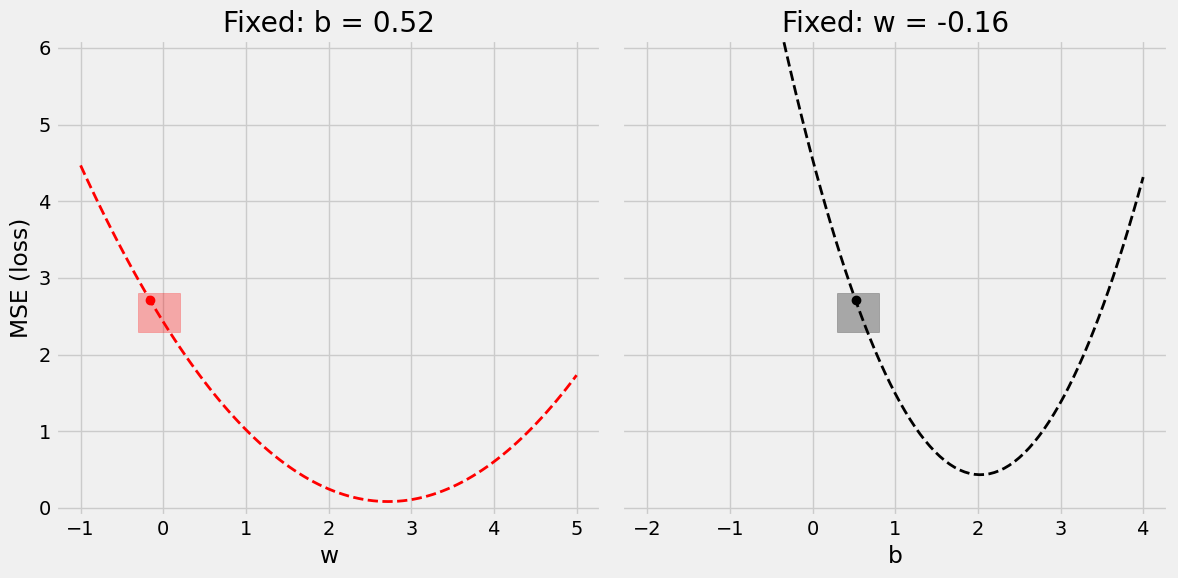
\includegraphics[width=\linewidth]{img/08}
	\end{center}
\end{frame}

\begin{frame}{Regression Problem}
	\begin{center}
		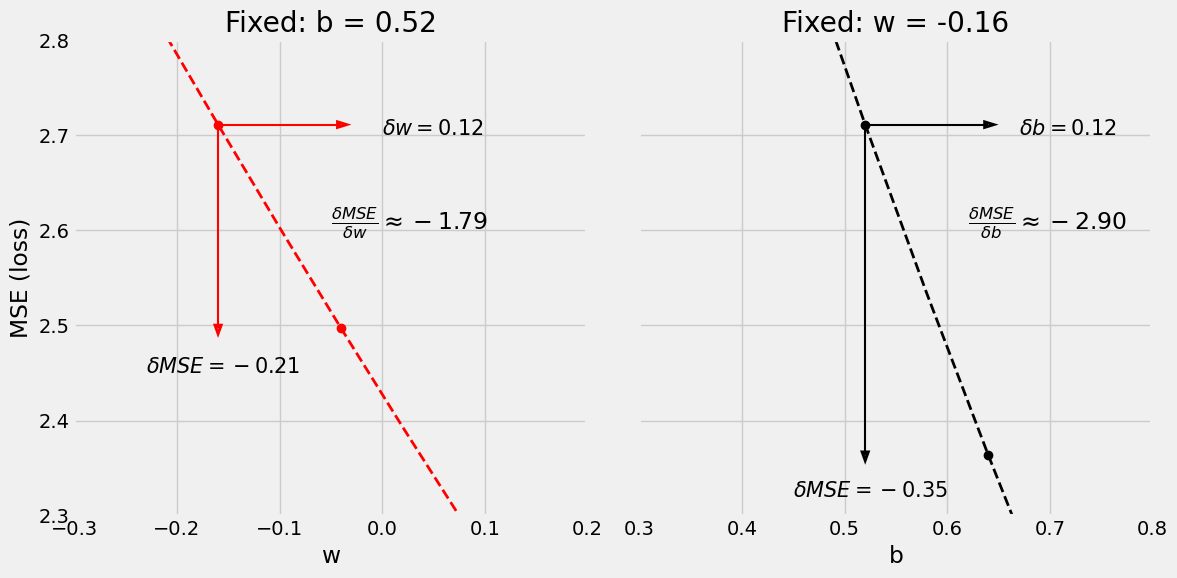
\includegraphics[width=\linewidth]{img/09}
	\end{center}
\end{frame}

\begin{frame}{Regression Problem}
	\begin{itemize}
		\item Update the parameters
		$$
		\begin{aligned}
			b &= b - \eta \frac{\partial{\text{MSE}}}{\partial{b}}
			\\
			w &= w - \eta \frac{\partial{\text{MSE}}}{\partial{w}}
		\end{aligned}
		$$
		$\eta$: learning rate
	\end{itemize}
\end{frame}

\begin{frame}{Regression Problem}
	\begin{itemize}
		\item low learning rate
		\begin{center}
			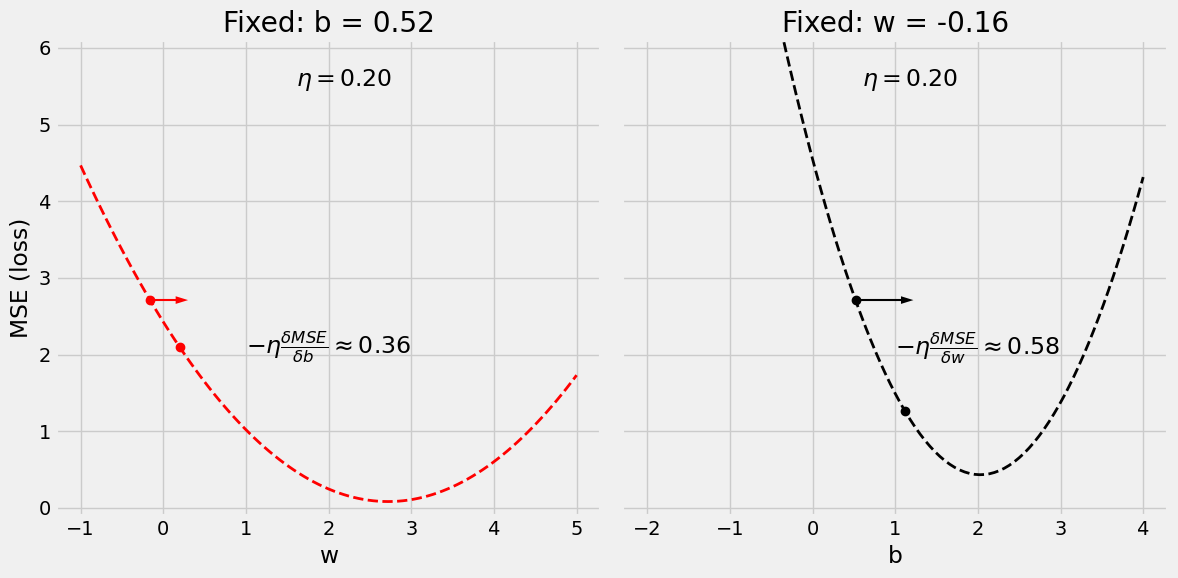
\includegraphics[width=\linewidth]{img/11}
		\end{center}
	\end{itemize}
\end{frame}

\begin{frame}{Regression Problem}
	\begin{itemize}
		\item high learning rate
		\begin{center}
			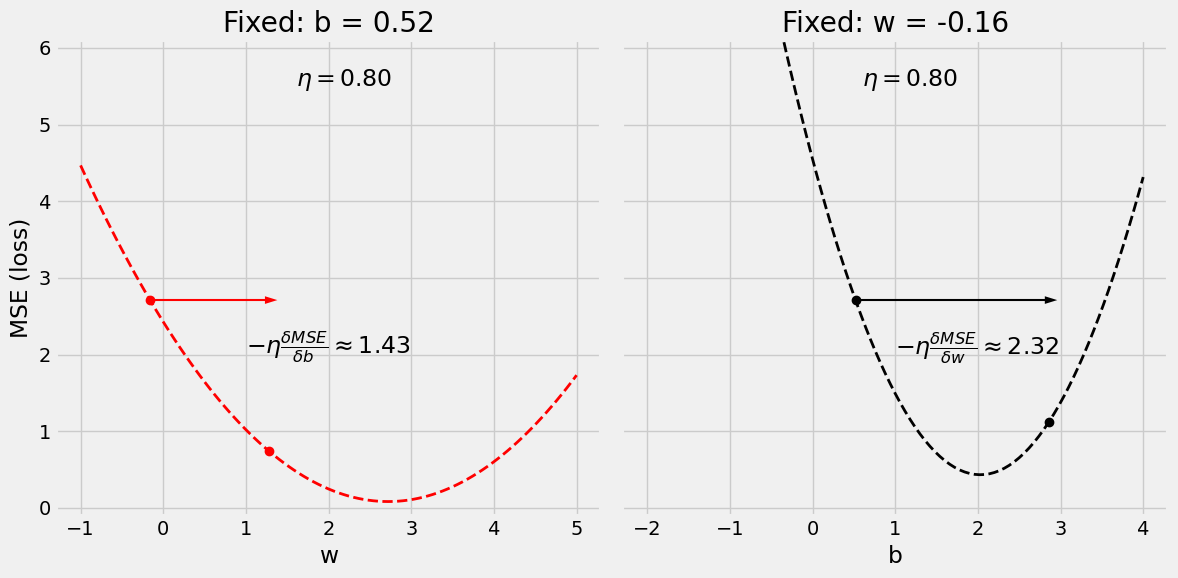
\includegraphics[width=\linewidth]{img/12}
		\end{center}
	\end{itemize}
\end{frame}

\begin{frame}{Regression Problem}
	\begin{itemize}
		\item very high learning rate
		\begin{center}
			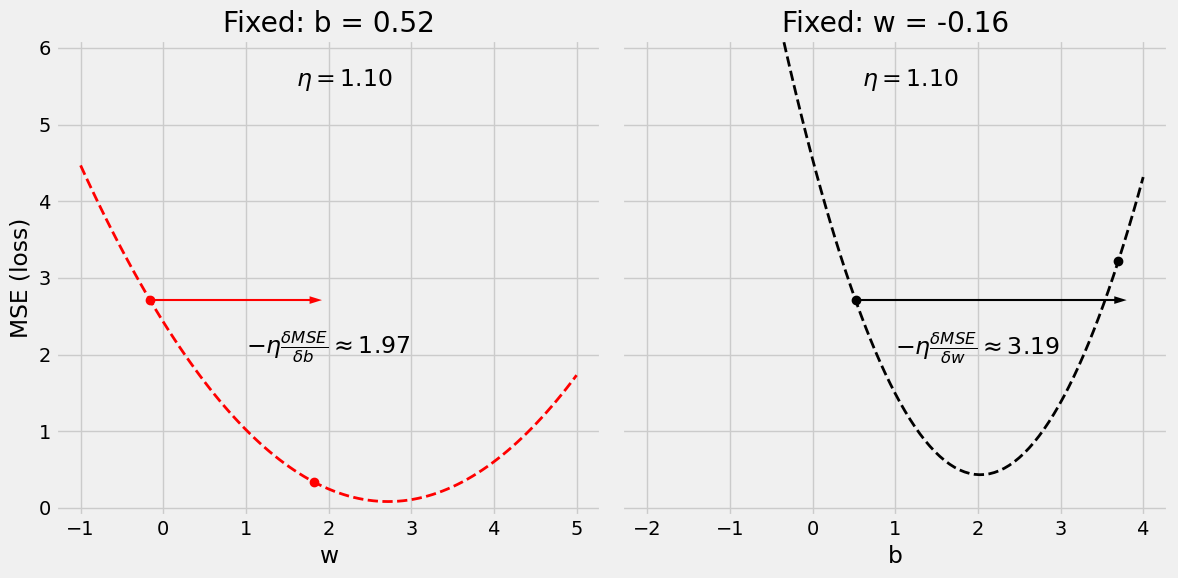
\includegraphics[width=\linewidth]{img/13}
		\end{center}
	\end{itemize}
\end{frame}

\begin{frame}{Regression Problem}
	\begin{center}
		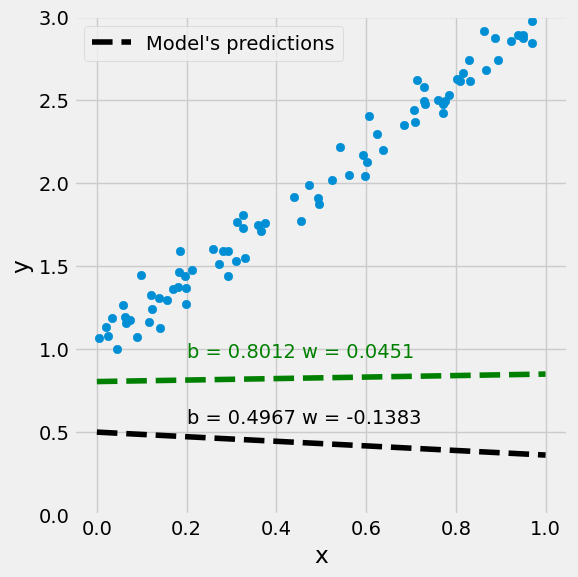
\includegraphics[width=0.6\linewidth]{img/10}
	\end{center}
\end{frame}

\begin{frame}{Regression Problem}
	\begin{itemize}
		\item Compute loss $\rightarrow$ Compute the gradients $\rightarrow$ update the parameters
		\item Repeat! 1000 epochs!
	\end{itemize}
	\begin{center}
		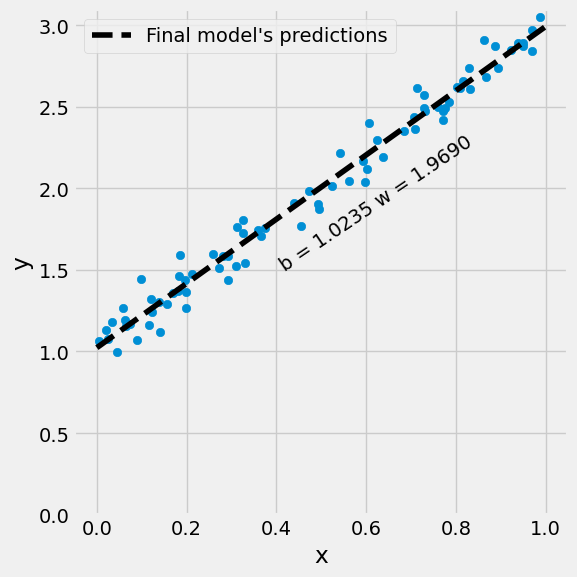
\includegraphics[width=0.5\linewidth]{img/14}
	\end{center}
\end{frame}

\begin{frame}{Classification Problem}
	\begin{center}
		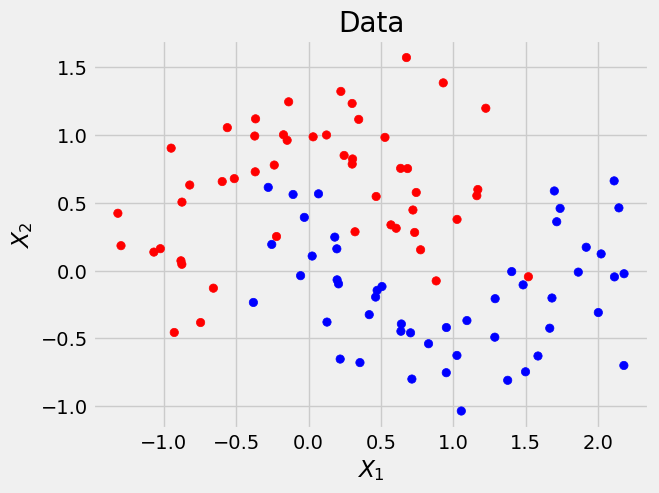
\includegraphics[width=0.6\linewidth]{img/17}
		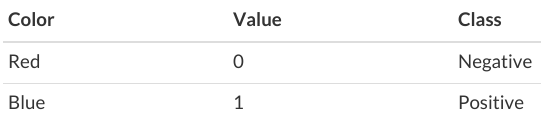
\includegraphics[width=0.6\linewidth]{img/18}
	\end{center}
\end{frame}

\begin{frame}{Classification Problem}
	\begin{itemize}
		\item A linear regression model with two features
		$$
		y = b + w_1x_1 + w_2x_2 + \epsilon
		$$
		\item Our labels ($y$) are discrete; that is, they are either zero or one; no other value is allowed. We need to change the model slightly to adapt it to our purposes
		$$
		y =
		\begin{cases}
			1,\ \text{if }b + w_1x_1 + w_2x_2 \ge 0
			\\
			0,\ \text{if }b + w_1x_1 + w_2x_2 < 0
		\end{cases}
		$$
	\end{itemize}
\end{frame}

\begin{frame}{Classification Problem}
	\begin{itemize}
		\item Logits ($z$)
		$$
		z = b + w_1x_1 + w_2x_2
		$$
		\item large positive logit values assigned to higher probabilities (of being in the positive class) and large negative logit values assigned to lower probabilities (of being in the positive class)
		$$
		\begin{aligned}
			& \text{P}(y=1) \approx 1.0, & \text{if } &z \gg 0
			\\
			& \text{P}(y=1) = 0.5, & \text{if } &z = 0
			\\
			& \text{P}(y=1) \approx 0.0, & \text{if } &z \ll 0
		\end{aligned}
		$$
	\end{itemize}
\end{frame}

\begin{frame}{Classification Problem}
	\begin{itemize}
		\item We still need to figure out a function that maps logit values into probabilities.
		\item Odds Ratio \& Log Odds Ratio
		\begin{align*}
			\text{odds ratio }(p) &= \frac{p}{q} = \frac{p}{1-p} \\
			\text{log odds ratio }(p) &= \text{log}\left(\frac{p}{1-p}\right)
		\end{align*}
		\begin{center}
			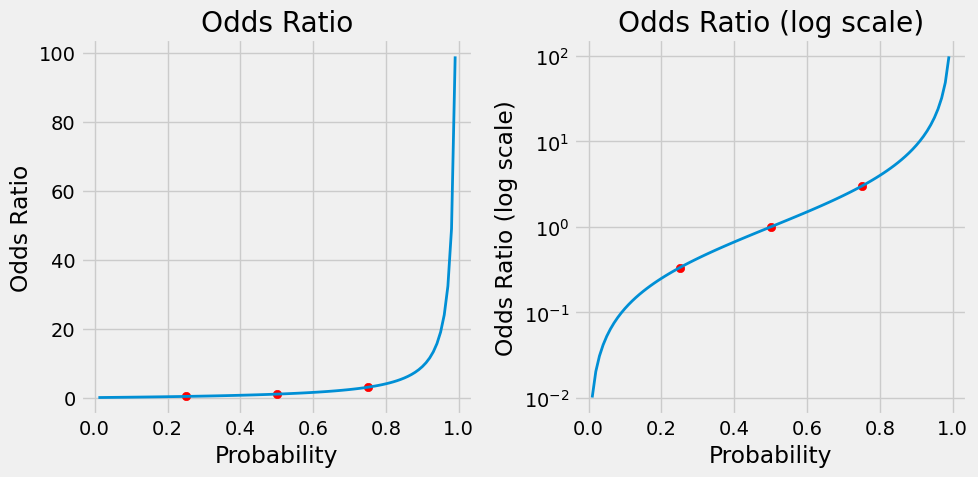
\includegraphics[width=0.7\linewidth]{img/19}
		\end{center}
	\end{itemize}
	\vfill\null
\end{frame}

\begin{frame}{Classification Problem}
	\begin{itemize}
		\item From Logits to Probabilities
		$$
		\begin{aligned}
			b + w_1x_1 + w_2x_2 = &\ z = \text{log}\left(\frac{p}{1-p}\right) \nonumber
			\\
			e^{b + w_1x_1 + w_2x_2} = &\ e^z = \frac{p}{1-p} \nonumber
		\end{aligned}
		$$
	\end{itemize}
\end{frame}

\begin{frame}{Classification Problem}
	\begin{itemize}
		\item From Logits to Probabilities
		$$
		\begin{aligned}
			\frac{1}{e^z}& = \frac{1-p}{p}
			\\
			e^{-z}& = \frac{1}{p} - 1
			\\
			1 + e^{-z}& = \frac{1}{p}&
			\\
			p& = \frac{1}{1 + e^{-z}}
		\end{aligned}
		$$
	\end{itemize}
\end{frame}

\begin{frame}{Classification Problem}
	\begin{itemize}
		\item From Logits to Probabilities
		$$
		p = \sigma(z) = \frac{1}{1+e^{-z}}
		$$
		\item That’s a sigmoid function!
		\begin{center}
			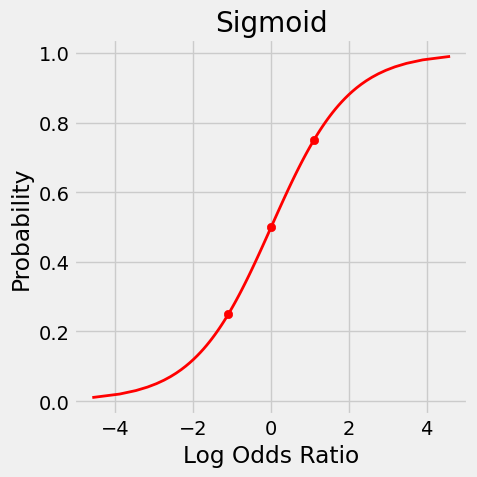
\includegraphics[width=0.5\linewidth]{img/20}
		\end{center}
	\end{itemize}
	\vfill\null
\end{frame}

\begin{frame}{Classification Problem}
	\begin{itemize}
		\item Logistic Regression
		\item Given two features, $x_1$ and $x_2$, the model will fit a linear regression such that its outputs are logits $(z)$, which are then converted into probabilities using a sigmoid function.
		$$
		\text{P}(y=1) = \sigma(z) = \sigma(b+w_1x_1+w_2x_2)
		$$
		\begin{center}
			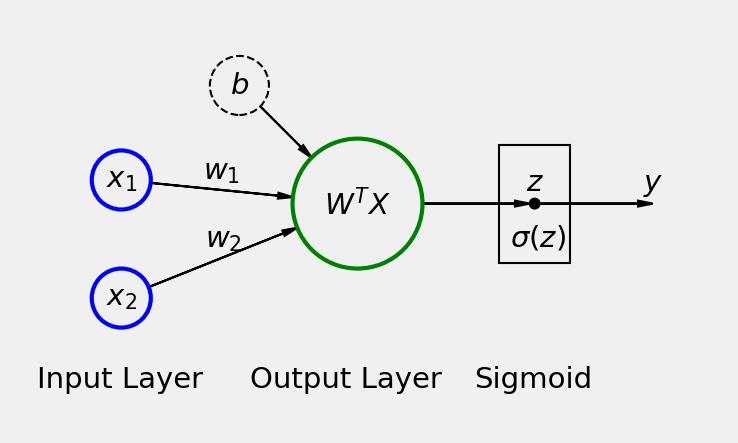
\includegraphics[width=0.6\linewidth]{img/21}
		\end{center}
	\end{itemize}
	\vfill\null
\end{frame}

\begin{frame}{Classification Problem}
	$$
	W =
	\underset{(3 \times 1)}{
		\begin{bmatrix}
			b \\
			w_1 \\
			w_2
	\end{bmatrix}};
	X = 
	\underset{(3 \times 1)}{
		\begin{bmatrix}
			1 \\
			x_1 \\
			x_2
	\end{bmatrix}}
	$$
	$$
	\begin{aligned}
		z
		& = W^T X
		=
		\underset{(1 \times 3)}{
			\begin{bmatrix}
				- & w^{T} & -\\
		\end{bmatrix}}
		\underset{(3 \times 1)}{
			\begin{bmatrix}
				1 \\
				x_1 \\
				x_2
		\end{bmatrix}}
		= \underset{(1 \times 3)}{
			\begin{bmatrix}
				b & w_1 & w_2
		\end{bmatrix}}
		\underset{(3 \times 1)}{
			\begin{bmatrix}
				1 \\
				x_1 \\
				x_2
		\end{bmatrix}}\\
		& = b + w_1x_1 + w_2x_2
	\end{aligned}
	$$
\end{frame}

\begin{frame}{Classification Problem}
	\begin{itemize}
		\item Loss:
		\item Error for a data point in the positive class:
		$$
		y_i = 1 \Rightarrow \text{error}_i=\text{log}(\text{P}(y_i=1))
		$$
		\item Probability of a data point’s belonging to the negative class:
		$$
		\text{P}(y_i=0)=1-\text{P}(y_i=1)
		$$
		\item Error for a data point in the negative class
		$$
		y_i = 0 \Rightarrow \text{error}_i=\text{log}(1-\text{P}(y_i=1))
		$$
	\end{itemize}
\end{frame}

\begin{frame}{Classification Problem}
	\begin{itemize}
		\item Once all errors are computed, they are aggregated into a loss value.
		\item For the \textbf{binary-cross entropy loss}, we simply take the average of the errors and invert its sign.
		\small
		$$
		\text{BCE}(y)={-\frac{1}{(N_{\text{pos}}+N_{\text{neg}})}\Bigg[{\sum_{i=1}^{N_{\text{pos}}}{\text{log}(\text{P}(y_i=1))} + \sum_{i=1}^{N_{\text{neg}}}{\text{log}(1 - \text{P}(y_i=1))}}\Bigg]}
		$$
		$$
		\text{BCE}(y)={-\frac{1}{N}\sum_{i=1}^{N}{\left[y_i \text{log}(\text{P}(y_i=1)) + (1-y_i) \text{log}(1-\text{P}(y_i=1))\right]}}
		$$
	\end{itemize}
\end{frame}

\begin{frame}{Classification Problem}
	\begin{itemize}
		\item Compute loss $\rightarrow$ Compute the gradients $\rightarrow$ update the parameters
		\item Repeat! 1000 epochs!
	\end{itemize}
	\begin{center}
		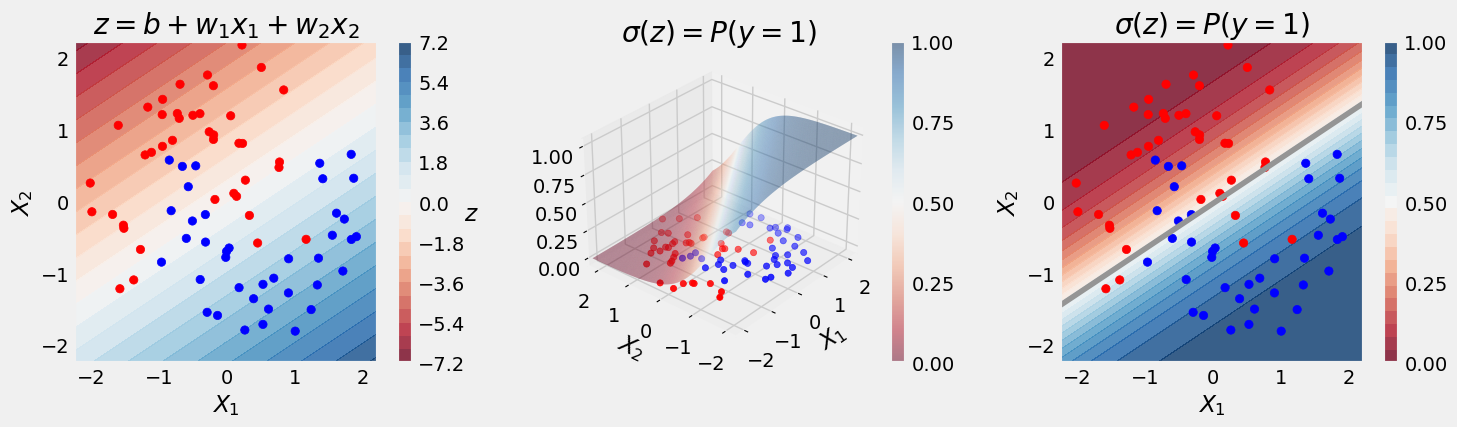
\includegraphics[width=\linewidth]{img/22}
	\end{center}
\end{frame}


\end{document}
